\documentclass[tikz]{standalone}

\begin{document}
	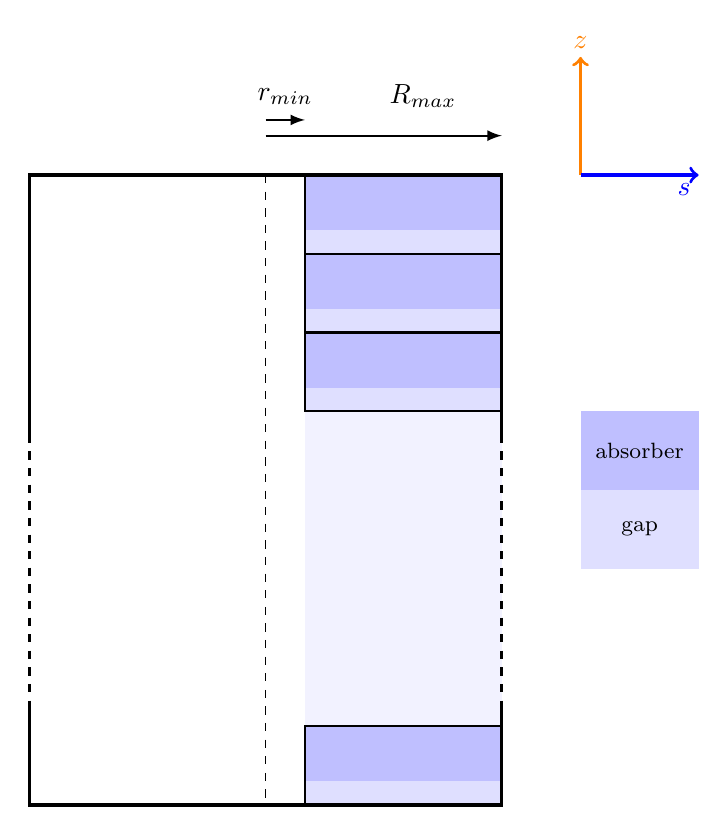
\begin{tikzpicture}
		\fill [blue!50, nearly transparent] (0.5,3) rectangle (3,3.3);
		\fill [blue!50, semitransparent] (0.5,3.3) rectangle (3,4);
		
		\fill [blue!50, nearly transparent] (0.5,2) rectangle (3,2.3);
		\fill [blue!50, semitransparent] (0.5,2.3) rectangle (3,3);
		
		\fill [blue!50, nearly transparent] (0.5,1) rectangle (3,1.3);
		\fill [blue!50, semitransparent] (0.5,1.3) rectangle (3,2);
		
		\fill [blue!50, nearly transparent] (0.5,-4) rectangle (3,-3.7);
		\fill [blue!50, semitransparent] (0.5,-3.7) rectangle (3,-3);
		
		\fill [blue!50, very nearly transparent] (0.5,-3) rectangle (3,1);
				
		\draw [very thick] (3, 0.7) -- (3,4) -- (-3,4) -- (-3,0.7);
		\draw [very thick, dashed] (-3,0.7) -- (-3,-2.7);
		\draw [very thick, dashed] (3,0.7) -- (3,-2.7);
		\draw [very thick] (-3,-2.7) -- (-3,-4) -- (3,-4) -- (3,-2.7);
		
		\draw [dashed] (0,4) -- (0,-4);
		
		\draw [thick] (0.5,3) rectangle (3,4);
		\draw [thick] (0.5,2) rectangle (3,3);
		\draw [thick] (0.5,1) rectangle (3,2);
		\draw [thick] (0.5,-4) rectangle (3,-3);
		
		\fill [blue!50, semitransparent] (4,0) rectangle (5.5,1);
		\node at (4.75, 0.5) {\footnotesize absorber};
		\fill [blue!50, nearly transparent] (4,-1) rectangle (5.5,0);
		\node at (4.75, -0.5) {\footnotesize gap};
		
		\draw [thick, -latex] (0,4.5) -- (3,4.5);
		\node at (2, 5) {$R_{max}$};
		\draw [thick, -latex] (0,4.7) -- (0.5,4.7);
		\node at (0.25, 5) {$r_{min}$};

		\draw[orange,very thick, ->] (4,4) -- (4,5.5) node[above=-1]{$z$};
		\draw[blue,very thick, ->] (4,4) -- (5.5,4) node[below left=-1]{$s$};
	\end{tikzpicture}
\end{document}